\begin{document}
\maketitle

\begin{frame}
  \titlepage
\end{frame}

\cleardoublepage

\tableofcontents

\cleardoublepage

\section{Introduction}

\begin{frame}{DBIx::Class Training}
\note{
  Explain how I ended up doing DBIx::Class training.
}
\begin{figure}[!ht]
\centering
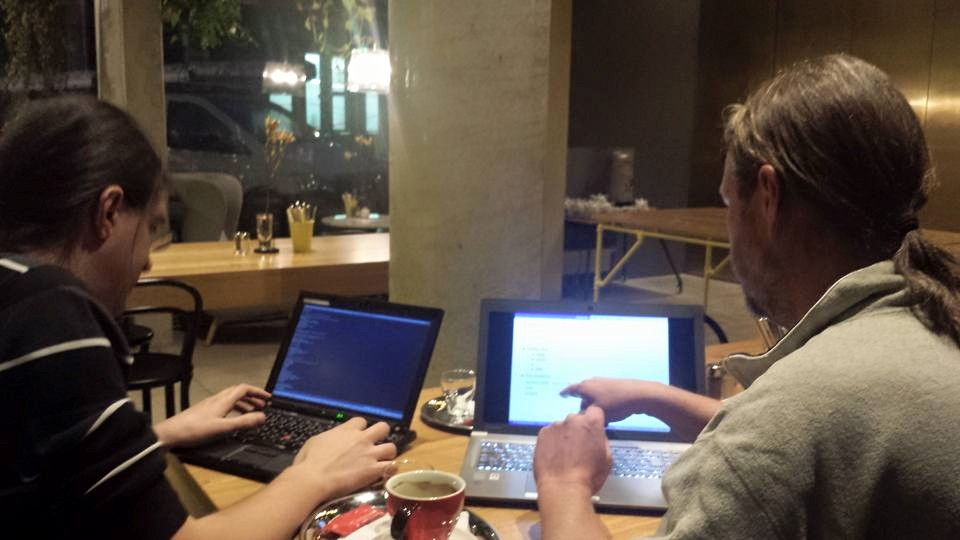
\includegraphics[width=1\linewidth]{img/training-preps.jpg}
\end{figure}
\end{frame}

\subsection{Best Thing Since Sliced Bread}

\begin{frame}{Best Thing Since Sliced Bread}

% https://en.wikipedia.org/wiki/Sliced_bread#/media/File:Brood.jpg

\begin{figure}[!ht]
\centering
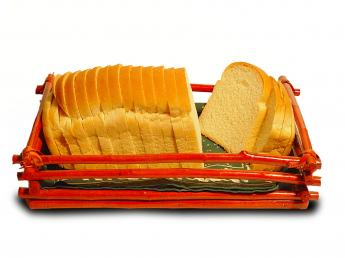
\includegraphics[width=1\linewidth]{img/sliced-bread.jpg}
\end{figure}
\end{frame}

\begin{frame}{Best Thing Since Sliced Bread}
\begin{itemize}
\item OO instead of SQL
\item Business Logic
\item Composability
\item Performance
\item Ecosystem
\end{itemize}
\end{frame}

\subsection{Can of Worms}

\begin{frame}{Can of Worms}
\begin{figure}[!ht]
\centering

\includegraphics[width=0.75\linewidth]{img/canofworms.png}
\end{figure}
\end{frame}

\begin{frame}{Can of Worms}
\begin{itemize}
\item SQL::Abstract
\item Class names (Result, ResultSet)
\item Documentation outline
\end{itemize}
\end{frame}

\subsection{DBIx::Class instead of SQL queries}

\begin{frame}{SQL is ...}
\begin{itemize}
\item SQL is ... boring
\item SQL is ... complex
\item SQL is ... governed by "15 competing standards"
\item SQL is ... not object oriented
\end{itemize}
\end{frame}


Using DBIx::Class allows you move all your business logic
into the database schema instead scattering it around a (web)
application.

\subsection{Business Logic}
\begin{frame}{Business Logic}
% move business logic into schema
% https://pixabay.com/en/gear-gears-euro-forex-dollar-384743/
\begin{figure}[!ht]
\centering

\includegraphics[width=0.75\linewidth]{img/business-logic.jpg}
\end{figure}
\end{frame}

\begin{frame}{Business Logic Benefits}
\begin{itemize}
\item Multiple Consumers
\begin{itemize}
\item Web application(s)
\item Cron jobs, scripts
\item Test environments
\end{itemize}
\item Hide Implementation
\begin{itemize}
\item SQL Dialects
\item Application View
\end{itemize}
\item Changes / DRY
\end{itemize}
\end{frame}

\subsection{Performance}

All the experience, tests and different areas in which 
DBIx::Class is applied makes it perform better than
handwritten SQL is most cases.

\begin{frame}{Performance}
\begin{itemize}
\item Experience
\item Test results
\item Use cases
\end{itemize}
\end{frame}
 
In case you feel that isn't correct, please call our hotline:

\begin{frame}
\begin{figure}[!ht]
\centering
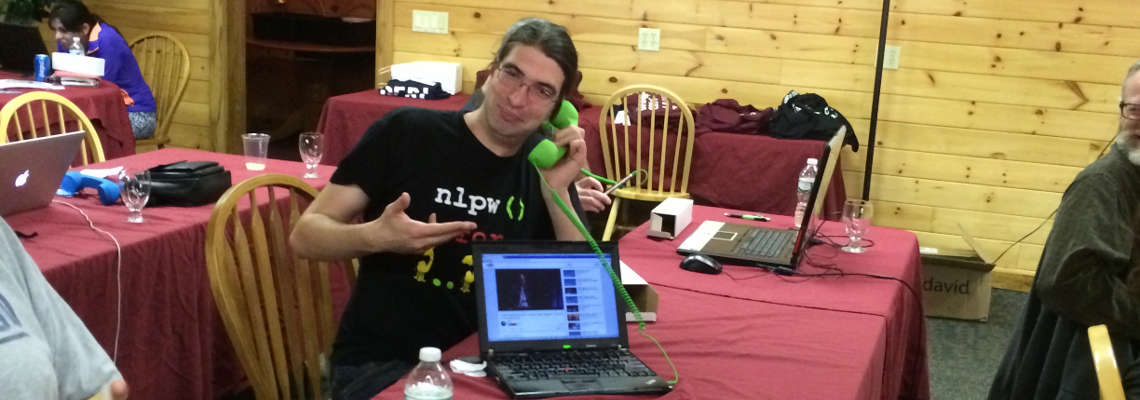
\includegraphics[width=1\linewidth]{img/perldance-2014-modern-tech.jpg}
\end{figure}
\end{frame}

But if you want to resort to SQL at some point, DBIx::Class allows you
to that too

\begin{frame}[fragile]{Literal SQL}
\begin{lstlisting}
$schema->resultset('PlaceVisited')->search(
{
  users_id => {
    -in => \[
       'SELECT users_id FROM users WHERE users_id > ?',
       2
    ]
  }
});
\end{lstlisting}
\end{frame}

But please don't complain if that leads to headache
and wasted time better spent on proper DBIx::Class
code.

\begin{frame}{SQL Headache}
% https://pixabay.com/en/stress-man-hand-flame-burn-fire-864141/
\begin{figure}[!ht]
\centering

\includegraphics[width=1\linewidth]{img/stress.jpg}
\end{figure}
\end{frame}

\section{SQL/OO}

\begin{frame}{From SQL to OO}
\begin{itemize}
\item SQL query
\item Turn into DBIx::Class search
\item Break it down
\end{itemize}
\end{frame}

\begin{frame}[fragile]{Simple SQL query}
List of talks on last day of Perl Dancer Conference:
\begin{lstlisting}
SELECT talks_id, author_id, conferences_id, duration,
title, tags, abstract, url, comments, accepted, confirmed, 
lightning, scheduled, start_time, room, survey_id 
FROM talks 
WHERE accepted is TRUE 
AND conferences_id = 1 
AND room != '' 
AND start_time >= '2015-10-22 00:00:00'
AND start_time <= '2015-10-23 00:00:00'
\end{lstlisting}
\end{frame}

\begin{frame}[fragile]{Simple SQL query}
With DBIx::Class:
\begin{lstlisting}
my $talks = $schema->resultset('Talk')->search(
    {
        accepted       => 1,
        conferences_id => 1,
        room           => { '!=' => '' },
        start_time     => {
            '>=' => '2015-10-22 00:00:00'
            '<=' => '2015-10-23 00:00:00'
            },
    },
);
\end{lstlisting}
\end{frame}

\section{Truth of ResultSet}
\note{
  If you hear the term ResultSet, you probably thing
  we are talking about a number of results aka
  table rows.
}

\begin{frame}{Truth of ResultSet}
\begin{figure}[!ht]
\centering
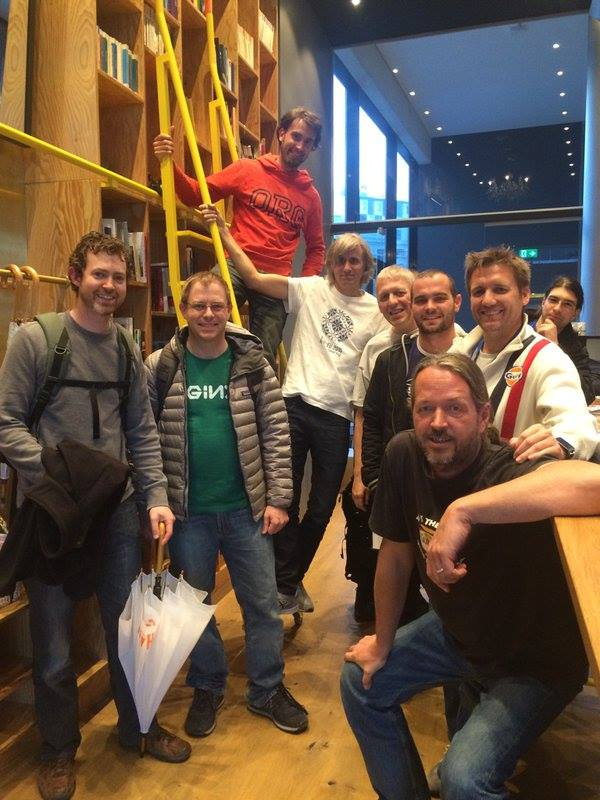
\includegraphics[width=0.5\linewidth]{img/pdc_users.jpg}
\end{figure}
\end{frame}

% https://pixabay.com/en/wrong-way-sign-road-caution-167535/

\begin{frame}{Truth of ResultSet}
\begin{figure}[!ht]
\centering

\includegraphics[width=1\linewidth]{img/wrong-way.jpg}
\end{figure}
\end{frame}

\begin{frame}[fragile]{Truth of ResultSet}
% \centering
\sout{ResultSet}

\begin{lstlisting}
isa(Query Plan);
\end{lstlisting}

\end{frame}

\begin{frame}[fragile]{Truth of ResultSet}

This doesn't execute SQL:

\begin{lstlisting}
my $talks = $schema->resultset('Talk')->search(...);
\end{lstlisting}

This does:

\begin{lstlisting}
my $first_talk = $schema->resultset('Talk')
                 ->search(...)->first;
\end{lstlisting}

\end{frame}

\section{Composability}

Composability means that you don't need to construct the
complete at once, but compose it together, e.g with
chaining.

The underlying mechanism is that \verb|->search| on a
ResultSet actually doesn't search.

\begin{frame}[fragile]{Talks}

\begin{lstlisting}
my $talks = $schema->resultset('Talk')->search(
    {
        accepted       => 1,
        conferences_id => 1,
        room           => { '!=' => '' },
        start_time     => {
            '>=' => '2015-10-22 00:00:00'
            '<=' => '2015-10-23 00:00:00'
            },
    },
);
\end{lstlisting}
\end{frame}

\begin{frame}[fragile]{Talks}

\begin{lstlisting}
my $talks = $schema->resultset('Talk')
   ->search({accepted       => 1})
   ->search({conferences_id => 1})
   ->search({room           => { '!=' => '' }),
   ->search({start_time     => {
            '>=' => '2015-10-22 00:00:00'
            '<=' => '2015-10-23 00:00:00'
            }}),
);
\end{lstlisting}
\end{frame}

\subsection{Predefined Search}
\begin{frame}[fragile]{Predefined Search}
\begin{lstlisting}
sub scheduled_for {
    my ( $self, $date ) = @_;

    $self->throw_exception("scheduled_for required arg date missing")
      unless defined $date;

    my $schema = $self->result_source->schema;

    $self->search({
        start_time     => {
            '>=' => $schema->format_datetime( $date ),
            '<=' =>
                $schema->format_datetime( $date->clone->add( days => 1 ) )
            },
    });
}
\end{lstlisting}
\end{frame}

\begin{frame}[fragile]{Predefined Search}
\begin{lstlisting}
sub scheduled_for {
    my ( $self, $date ) = @_;

    $self->throw_exception("scheduled_for required arg date missing")
      unless defined $date;

    my $schema = $self->result_source->schema;

    $self->search({
        start_time     => {
            '>=' => $schema->format_datetime( $date ),
            '<=' =>
                $schema->format_datetime( $date->clone->add( days => 1 ) )
            },
    });
}
\end{lstlisting}
\end{frame}

\begin{frame}[fragile]{Using predefined search}

\begin{lstlisting}
my $dt_date = DateTime->new(
    year => 2015,
    month => 10,
    day => 22,
);

my $talks = $schema->resultset('Talk')
   ->search({accepted       => 1})
   ->search({conferences_id => 1})
   ->search({room           => { '!=' => '' }),
   ->scheduled_for($dt_date);
);
\end{lstlisting}
\end{frame}

\begin{frame}[fragile]{Subjects included}
\begin{itemize}
\item Exceptions
\item Access main schema object
\item DateTime inflation
\item Schema::DateTime helper
\end{itemize}
\end{frame}

\section{Other Nice Stuff}

\begin{frame}{Other Nice Stuff}
\begin{itemize}
\note{Sugar for DBIx::Class}
\item Candy
\item Subclassing Schema
\end{itemize}
\end{frame}

\subsection{Candy - Sugar for DBIx::Class}

\begin{frame}{Sugar for DBIx::Class}
% https://pixabay.com/en/candy-cane-candy-cane-winter-488009/
\begin{figure}[!ht]
\centering

\includegraphics[width=0.8\linewidth]{img/candy-cane.jpg}
\end{figure}
\end{frame}

\begin{frame}[fragile]{Vanilla Result Class}
\begin{lstlisting}
package TravelDance::Schema::Result::Country;
use warnings;
use strict;
use base 'DBIx::Class::Core';

__PACKAGE__->table('countries');

__PACKAGE__->add_columns(
    country_iso_code => {
        data_type => "char",
        size      => 2,
    },
    name => {
        data_type => "varchar",
        size      => 255,
    },
);
\end{lstlisting}
\end{frame}

\begin{frame}[fragile]{Candy Result Class}
\begin{lstlisting}
package TravelDance::Schema::Result::Country;
use TravelDance::Schema::Candy;

primary_column country_iso_code => {
    data_type => "char",
    size      => 2
};

column name => {
    data_type => "varchar",
    size      => 255
};
\end{lstlisting}
\end{frame}

\subsection{Subclassing Schema}

You can also subclass schemas.

* add new columns to existing tables

\begin{frame}[fragile]{Subclass Example}
\begin{lstlisting}
package PerlDance::Schema;

use base 'Interchange6::Schema';

Interchange6::Schema->load_namespaces(
    default_resultset_class => 'ResultSet',
    result_namespace        =>
        [ 'Result', '+PerlDance::Schema::Result' ],
    resultset_namespace     =>
        [ 'ResultSet', '+PerlDance::Schema::ResultSet' ],
);
\end{lstlisting}
\end{frame}



\section{DBIx::Class Helpers}

\begin{frame}{DBIx::Class Helpers}
Simplify the common case stuff for DBIx::Class.
\end{frame}

\begin{frame}{DBIx::Class Helpers}
\begin{figure}[!ht]
\centering

\includegraphics[width=0.4\linewidth]{img/frew.png}
\caption{Arthur Axel "fREW" Schmidt}
\end{figure}
\end{frame}

% list of helpers we show

\begin{frame}{DBIx::Class Helpers}
\begin{itemize}
\item Quote Names
\item Me
\end{itemize}
\end{frame}

\subsection{Helper::QuoteNames}

\begin{frame}[fragile]{Helper::QuoteNames}
\begin{itemize}
\item Escaping reserved words
\item Differ between engines and version
\item e.g. MySQL
\begin{itemize}
\item \verb|select user from userdb| => crash
\item \verb|select `user` from `userdb`| => works
\end{itemize}
\item \verb|quote_names| in connection info
\end{itemize}
\end{frame}

\begin{frame}[fragile]{Helper::QuoteNames}
\begin{lstlisting}

package Interchange6::Schema;

use base 'DBIx::Class::Schema';

__PACKAGE__->load_components( 'Helper::Schema::QuoteNames' );

...

\end{lstlisting}
\end{frame}

\subsection{Helper::Resultset::Me}

Predefined queries present a problem: what is the table alias I need to use?
We can do:

\begin{frame}[fragile]{Helper::Resultset::Me}
\begin{lstlisting}
sub in_germany {
    my $self = shift;
    my $current_source_alias =
        $self->current_source_alias;
    return $self->search(
        { "$current_source_alias.country_iso_code"
          => 'DE' }
    );
}
\end{lstlisting}
\end{frame}

but using this helper makes things much simpler:

\begin{frame}[fragile]{Helper::Resultset::Me}
\begin{lstlisting}
sub in_germany {
    my $self = shift;


    return $self->search(
        { $self->me('country_iso_code') => 'DE' }
    );

}
\end{lstlisting}
\end{frame}

\subsection{Helper::ResultSet::Shortcut}



\note{A lot of shortcuts are provided, I'll show
you just a few examples.}

\begin{frame}{Shortcuts}
\begin{itemize}
\item columns
\item like
\item hri
\end{itemize}
\end{frame}

\begin{frame}[fragile]{columns Shortcut}

\verb|columns| shortcut:

\begin{lstlisting}
$rs->columns([qw/ first_name last_name /]);
\end{lstlisting}

equivalent to:

\begin{lstlisting}
$rs->search( undef, { 
    columns => [qw/ first_name last_name /] 
} );
\end{lstlisting}
\end{frame}

\begin{frame}[fragile]{like Shortcut}

\verb|like| shortcut:

\begin{lstlisting}
$rs->like( 'city', 'region', '%York' );
\end{lstlisting}

or:

\begin{lstlisting}
$rs->like([ 'city', 'region' ], '%York' );
\end{lstlisting}

equivalent to:

\begin{lstlisting}
$rs->search(
    { city => { -like => '%York' },
    { region => { -like => '%York' },
);
\end{lstlisting}
\end{frame}

\begin{frame}[fragile]{hri Shortcut}

\verb|hri| shortcut:

\begin{lstlisting}
$rs->hri;
\end{lstlisting}

equivalent to:

\begin{lstlisting}
$rs->search( undef, {
    result_class => 
        'DBIx::Class::ResultClass::HashRefInflator'
});
\end{lstlisting}
\end{frame}

\subsection{Helper::Row::OnColumnChange}

\begin{frame}[fragile]{Helper::Row::OnColumnChange}

Do things when the value of a column changes.

\begin{itemize}
\item before\_column\_change
\item around\_column\_change
\item after\_column\_change
\end{itemize}

\end{frame}

\begin{frame}[fragile]{Helper::Row::OnColumnChange}

\begin{lstlisting}
package TravelDance::Schema::Result::User;

use TravelDance::Schema::Candy -components =>
    [qw(Helper::Row::OnColumnChange 
        InflateColumn::DateTime)];

use DateTime;

column last_password_change => {
    data_type => timestamp,
};
\end{lstlisting}
\end{frame}

\begin{frame}[fragile]{Helper::Row::OnColumnChange}

On password change:

\begin{itemize}
\item check new password against old one
\item update \verb|last_password_change| column
\end{itemize}

\end{frame}

\begin{frame}[fragile]{Helper::Row::OnColumnChange}
\begin{lstlisting}
after_column_change password => {
    method   => 'change_password',
    txn_wrap => 1,  # wrap it all in a transaction
};
\end{lstlisting}
\end{frame}

\begin{frame}[fragile]{Helper::Row::OnColumnChange}
\begin{lstlisting}
sub change_password {
    my ( $self, $old_value, $new_value ) = @_;
    if ( $self->check_password($new_value) ) {
        $self->throw_exception("Password not changed")
    }
    else {
        $self->update(
            { last_password_change => DateTime->now() }
        );
    }
}
\end{lstlisting}
\end{frame}

\subsection{Helper::Schema::DateTime}

\begin{frame}[fragile]{Helper::Schema::DateTime}
VisitedPlaces visited in the last year:

\begin{lstlisting}
my $one_year_ago = $schema->format_datetime(
    DateTime->now->subtract( year => 1 )
);

my $rs = $schema->resultset('PlaceVisited')->search(
    {
        visited => { '>' => $one_year_ago }
    }
);
\end{lstlisting}
\end{frame}

\begin{frame}[fragile]{Helper::Schema::DateTime}

Without the helper:

\begin{lstlisting}
my $dtf = $schema->storage->datetime_parser; # boilerplate
my $one_year_ago = $dtf->format_datetime(
    DateTime->now->subtract( year => 1 )
);

my $rs = $schema->resultset('PlaceVisited')->search(
    {
        visited => { '>' => $one_year_ago }
    }
);
\end{lstlisting}
\end{frame}

\subsection{HashRefInflator}

Using the HashRefInflator makes sense when you need to quickly retrieve
data from a massive resultset or you need a list of hash references anyway,
e.g. for input to a template in a web application.

\begin{frame}[fragile]{HashRefInflator}
\begin{lstlisting}
my $rs = $schema->resultset('Country')->search({}, {
   result_class
     => 'DBIx::Class::ResultClass::HashRefInflator',
 });
\end{lstlisting}
\end{frame}

\begin{frame}[fragile]{HashRefInflator with HRI helper}
\begin{lstlisting}
my $rs = $schema->resultset('Country')->search({})->hri;

# since 'search' here is redundant we can just use:
my $rs = $schema->resultset('Country')->hri;
\end{lstlisting}
\end{frame}

\subsection{Other useful helpers}
\begin{frame}{DBIx::Class Helpers}
\begin{itemize}
\item Random
\item RemoveColumns
\note{Easily correlate your ResultSets}
\item Helper::ResultSet::CorrelateRelationship
\note{Force numeric context on numeric columns:}
\item Helper::Row::NumifyGet
\end{itemize}
\end{frame}

% \section{Writing Tests}
% \begin{frame}{Writing Tests}
% \end{frame}

\section{Deployment Handler}

\subsection{Deploy/Upgrade/Downgrade}

\begin{frame}{Deployment Handler}
\begin{itemize}
\item DBIx::Class::DeploymentHandler
\item Deploy databases
\item Upgrade databases
\item Downgrade databases
\end{itemize}
\end{frame}

\subsection{Principles}

\begin{frame}{Principles}
\begin{itemize}
\item Create backup
\item Change schema
\item Add custom scripts
\item Bump version number
\item Prepare upgrade
\item Deploy upgrade
\end{itemize}
\end{frame}

Note: create backup can be done by DeploymentHandler itself.

\subsection{Change Schema}

\begin{frame}{Change Schema}
\begin{itemize}
\item Add table
\item Add column
\item Alter column
\end{itemize}
\end{frame}

\subsection{Bump version number}
\begin{frame}{Bump version number}
\begin{itemize}
\item Natural number => 1
\item Increase by 1 => 2
\end{itemize}
\end{frame}

\begin{frame}[fragile]{Version 1}
\begin{lstlisting}
package TravelDance::Schema;
use warnings;
use strict;
use base 'DBIx::Class::Schema';

our $VERSION = 1;

__PACKAGE__->load_namespaces();

1;
\end{lstlisting}
\end{frame}

\begin{frame}[fragile]{Version 2}
\begin{lstlisting}
package TravelDance::Schema;
use warnings;
use strict;
use base 'DBIx::Class::Schema';

our $VERSION = 2;

__PACKAGE__->load_namespaces();

1;
\end{lstlisting}
\end{frame}

\subsection{Prepare upgrade}

\begin{frame}[fragile]{Prepare upgrade}
\begin{lstlisting}
my $dh     = DBIx::Class::DeploymentHandler->new(
    {
        schema              => $schema,
        databases           => 'MySQL',
        sql_translator_args => { add_drop_table => 0 }
    }
);
$dh->prepare_deploy;
$dh->prepare_upgrade(
    {
        from_version => $dh->database_version,
        to_version => $dh->schema_version
    }
);
\end{lstlisting}
\end{frame}

\subsection{Add custom scripts}

\begin{frame}{Add custom scripts}
\begin{itemize}
\item Deployment
\item All upgrades
\item Specific upgrade
\end{itemize}
\end{frame}

\begin{frame}{Add custom scripts}
\begin{itemize}
\item Populate records on deployment
\item Add initial values for new tables
\begin{itemize}
\item hardcoded in script
\item from file
\end{itemize}
\end{itemize}
\end{frame}

\subsection{Internals}

Reference for directory layout:
\href{https://metacpan.org/pod/DBIx::Class::DeploymentHandler::DeployMethod::SQL::Translator}{DBIx::Class::DeploymentHandler::DeployMethod::SQL::Translator}

\begin{frame}[fragile]{Directories and files}
\begin{description}
\item[sql/PostgreSQL] SQL scripts for deploy and update
\item[sql/\_common] Custom scripts
\begin{description}
\item[sql/\_common/upgrade/\_any] All upgrades
\item[sql/\_common/upgrade/ 1-2] Upgrade from 1 to 2
\end{description}
\item[sql/\_deploy] Structure files (YAML)
\end{description}
\end{frame}

\section{Conclusion}

\subsection{Starting with DBIx::Class}

You can use \verb|dbicdump| to create a ``boilerplate'' schema from the
existing database.

\begin{frame}[fragile]{dbicdump}
\begin{lstlisting}
dbicdump -o dump_directory=/home/dance/TravelDance/lib 
         TravelDance::Schema 
         dbi:Pg:dbname=perldance
\end{lstlisting}
\end{frame}

\end{document}

%%% Local Variables: 
%%% mode: latex
%%% TeX-master: t
%%% End: 
